\chapter{HAK DAN KEWAJIBAN PEMBIMBING, PENGUJI DAN MAHASISWA
DALAM PEKERJAAN PROYEK POLITEKNIK POS INDONESIA}

\section{Aturan	Baru}
Kesepakatan	program	Studi untuk	Bobot	Nilai	adalah	sebagai	berikut:

\begin{table}[H]
\label{anjay}
\begin{tabular}{lll}
Pembimbing &  & : 65\% \\
Penguji &  & : 35\%
\end{tabular}
\end{table}

\section{Hak	dan	Kewajiban	Pembimbing}
\begin{enumerate}
\item Pembimbing	 berhak	 sepenuhnya	 menyetujui	 atau	 menolak	 mahasiswa	 bimbingannya	untuk	mengikuti	siding .
\item Pembimbing	harus	mendampingi	mahasiswa	selama	sidang	berlangsung .
\item Pembimbing	 diharuskan	 memberikan	 nilai	 Evaluasi	 Pelaksanaan Proyek	 sebelum	mahasiswa	bimbingannya	siding .
\item Pembimbing	 tidak	 diperkenankan	 menjawab	 pertanyaan	 Penguji	 untuk	 Mahasiswa,	kecuali	diminta	oleh	Penguji .
\item Pembimbing	berpakaian	rapi	dan	berdasi	selama	sidang.
\end{enumerate}

\section{Hak	dan	Kewajiban	Penguji}
\begin{enumerate}
\item Penguji	harus	sudah	datang	15	menit	sebelum	sidang	Proyek	dimulai.
\item Penguji	yang	terlambat	lebih	dari	15	menit	dari	waktu	sidang	yang	telah	ditetapkan	akan	
digantikan	oleh	Penguji	Pengganti.
\item Bila	tidak	ada	alasan	yang	kuat	atas	ketidak	hadiran	Penguji,	maka	Surat	Tugas	dan	Honor	
akan	dialihkan	kepada	Penguji	Pengganti.
\item Tim	Penguji	berhak	membatalkan	sidang	jika	Mahasiswa	terlambat	atau	tidak	hadir	sesuai	
jadwal	yang	telah	ditetapkan.
\item Tim	 penguji	 berhak	 membatalkan	 sidang,	 apabila	 pernyataan	 pembimbing	 tidak	 benar	(Tulisan	selesai	100\%	dan	Materi	Proyek	$\geq90\%$).
\item Sidang	akan	tetap	berlangsung	bila	2	(dua)	Penguji	(Ketua	Penguji	dan	Anggota	Penguji)	
hadir.
\item Berdasarkan	 proses	 sidang,	 Tim	 Penguji	 berhak	 sepenuhnya	 menetapkan	 status	 akhir	
sidang	tersebut,	yaitu	LULUS/LULUS	BERSYARAT/TIDAK	LULUS.
\item Ketua	 Penguji	 	 dan	 Anggota	 Penguji	 harus	 memberikan	 nilainya	 diakhir	 sidang	 secara	
objektif	dengan	tidak	melihat	Nilai	yang	diberikan	oleh	Penguji/Pembimbing	lain.
\item Ketua	 Penguji	 harus	 menghitung	 diakhir	 sidang	 Nilai	 Akhir	 yang	 dikumpulkan	 secara	
serentak	dari	Seluruh	Penguji	dan	Pembimbing	dengan	menggunakan	aturan/rumus	yang	
telah	ditetapkan.
\item Ketua	 Penguji	 harus	 mengkoordinasikan	 perbedaan	 nilai	 antar	 Penguji	 melalui	 proses	
debat/forum	diskusi	agar	didapat	nilai	yang	objektif	(Setiap	nilai	harus	berada	pada	range	
yang	sama,	misal	A,	B,	atau	C).
\item Ketua	Penguji	harus	mengumumkan	Nilai	Akhir	kepada	Mahasiswa	selesai	siding.
\item Penguji	berpakaian	rapi	dan	berdasi.
\end{enumerate}

\section{Hak	Dan	Kewajiban	Mahasiswa	Peserta	Sidang}
\begin{enumerate}
\item Mengikuti	jadwal	sidang	Proyek	oleh	Panitia.
\item Menyerahkan	 Surat	 Persetujuan	 Sidang	 dari	 Pembimbing	 sesuai	 waktu	 yang	 telah	
ditetapkan	oleh	Panitia.
\item Menyerahkan	 draf	 Laporan	 Proyek	 yang	 akan	 disidangkan	 kepada	 para	 penguji	 paling	
lambat	1	(satu)	hari	sebelum	sidang	dilaksanakan.
\item Hadir	30	menit	sebelum	sidang	dimulai.
\item Mempersiapkan	peralatan	sidang	yang	dibutuhkan.
\item Memakai	pakaian	seragam	dan	jas	almamater.
\item Berhak	mendapatkan	hasil	Evaluasi	Sidang	dari	tim	Penguji.
\end{enumerate}

\section{Prosedur Pelaksanaan	Sidang	Proyek	}
\begin{enumerate}
\item Waktu	pelaksanaan	sidang	1,5	jam	untuk	setiap	judul.
\item Sidang	dipimpin	oleh	Ketua	Penguji	(Pembimbing).
\item Pelaksanaan	sidang	sebagai	berikut :
	\begin{enumerate} [label=(\alph*)]
		\item Pembukaan	oleh	Ketua	Penguji. 
		\item Presentasi	Proyek	oleh	Mahasiswa		(maks.	15	menit).
		\item Demonstrasi	alat	dan	Tanya-jawab	(maks.	60	menit).
		\item Rapat	tertutup	penentuan	dan	diskusi	nilai	Tim	Penguji	(maks.	15	menit).
	\end{enumerate}
\end{enumerate}

\begin{figure}[H]
    \centering
    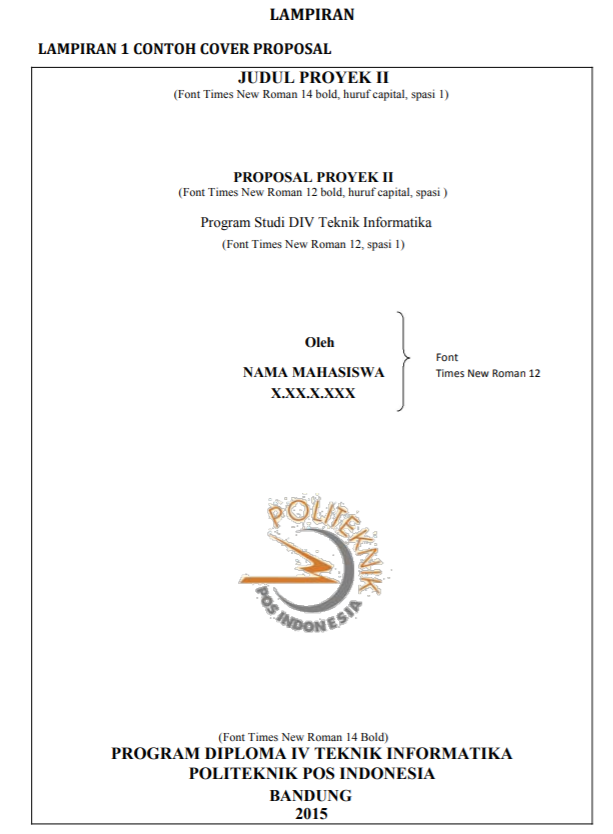
\includegraphics[scale=0.9]{figures/lap1.png}
    \label{alir}
\end{figure}

\begin{figure}[H]
    \centering
    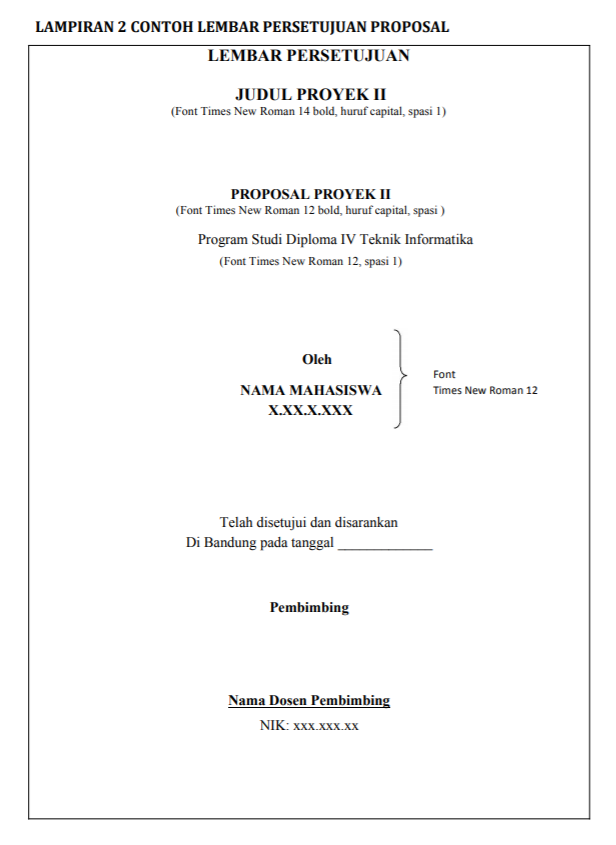
\includegraphics[scale=0.9]{figures/lap2.png}
    \label{alir}
\end{figure}